%  !TeX  root  =  user_guide.tex

\section{Модуль GDAL Tools}\label{label_plugingdaltools}

% when the revision of a section has been finalized,
% comment out the following line:
% \updatedisclaimer

\subsection{Что такое GDAL Tools?}\label{whatsgdal}
<<GDAL~Tools>>~--- это модуль, предоставляющий графический интерфейс к набору
инструментов Geospatial Data Abstraction Library, \url{http://gdal.osgeo.org}.
В него входят инструменты, позволяющие работать с широким спектром растровых
форматов: получать информацию о растрах, перепроецировать, объединять.
Также включены инструменты для создания векторных слоев изолиний,
получения отмывки рельефа на основе цифровой модели рельефа и создания виртуального растра VRT (Virtual Raster
Tile в формате XML)) из набора растровых файлов. Все перечисленные инструменты
становятся доступны, когда модуль установлен и загружен.

\subsection{Библиотека GDAL}\label{gdal_lib}
Библиотека GDAL состоит из набора программ, работающих из командной строки,
каждая с большим набором опций. Пользователи, которым комфортно работать в
командной строке, могут предпочесть ее, в том числе из-за полного набора
опций. Модуль <<GDAL Tools>> обеспечивает простой интерфейс к этим утилитам,
но с ограниченным набором наиболее востребованных опций.

{\setlength{\extrarowheight}{15pt}
\begin{longtable}{|p{3cm}|p{13cm}|}
\caption{Список инструментов GDAL Tools}\label{tab:gdaltools} \\
\hline Создать виртуальный растр (каталог) & Программа создает VRT
 (виртуальный набор данных), который представляет собой мозаику из исходных растров. \\
\hline Создать изолинии & Программа создает векторный файл изолиний из
 исходного растра цифровой модели рельефа (ЦМР).\\
\hline Растеризация &  Программа превращает векторный объекты (точечные,
 линейние и полигональные) в растровый слой (слои) существующего растра.
 Вектор может быть представлен в любом формате, поддерживаемом OGR. Обратите
 внимание, что векторный слой должен быть в той же системе координат, что и
 растр; перепроецирование <<на лету>> не поддерживается.\\
\hline Преобразовать в полигоны & Программа преобразует пикселы в полигоны,
 объединяя в один полигон примыкающие пикселы с одинаковым значением. Для
 каждого полигона в атрибутивной таблице указано значение пикселов исходного
 растра. Программа создаст новый векторный файл или перезапишет имеющийся,
 по умолчанию используется формат шейп-файла.\\
\hline Объединение &  Программа автоматически создает мозаику из набора растров.
 Все растры должны быть в одной системе координат и иметь одинаковое
 число каналов. Растры, тем не менее, могут иметь области перекрытия и разное
 пространственное разрешение. В областях перекрытия растры, идущие последними в
 списке, будут перекрывать идущие первыми. \\
\hline Отсеивание & Скрипт gdal\_sieve.py удаляет растровые полигоны размером
 меньше порогового (размер указывается в пикселах) и заменяет значения этих
 пикселей значением из наибольшего примыкающего растрового полигона. Результат
 может быть сохранен в канал существующего растра или в новый файл.\\
\hline Карта близости & Скрипт gdal\_proximity.py создает растровую карту
 близости, которая показывает расстояние от центра каждого пиксела до центра
 ближайшего пиксела с указанными пользователем значениями. Целевые пикселы
 выбираются в том же самом растре.\\
\hline Сбросить в черный & Программа анализирует изображение и попытается
 обозначить все пикселы, значения которых близки к совершенно черным (или
 совершенно белым)) и которые расположены вокруг совершенно черных (или белых)
 пикселей. Данная операция часто используется для <<исправления>> сжатых с
 потерями аэрофотоснимков, для того чтобы почти черные (или почти белые)
 пикселы могли быть интерпретированы как прозрачные (как пикселы <<нет данных>>)
 при создании мозаик.\\
\hline Трансформировать проекцию & Утилита gdalwarp используется для
 перепроецирования растров и создания мозаик. Программа перепроецирует растры
 в любую поддерживаемую проекцию, и может быть использована для трансформирования
 необработанного снимка с набором контрольных точек (GCP). \\
\hline Интерполяция & Программа строит растровый грид из доступных посредством
 OGR-источников данных. Исходные данные будут интерполированы для вычисления
 значений всех ячеек грида, и вы можете выбрать метод интерполяции из нескольких
 имеющихся.\\
\hline Преобразование форматов & Утилита gdal\_translate (преобразование
 форматов) может быть использована для конвертации растров из одного формата в
 другой, с возможностью использования операций обрезки, пересчета или изменения
 разрешения в процессе преобразования.\\
\hline Информация & Программа показывает разнообразную информацию о растре
 любого формата, поддерживаемого GDAL. \\
\hline Назначить проекцию &  Инструмент предназначен для назначения проекции
 растровым файлам. Может работать либо в пофайловом режиме, либо в пакетном (в таком
 случае указанная проекция прописывается для всех растров, расположенных в
 исходной директории). Поддерживаются все проекции, описанные в
 стандарте библиотеки PROJ.4. Если ваш растр имеет проекцию, которой нет в стандартном наборе, вам
 необходимо сначала описать ее и добавить в пользовательские. \\
\hline Построить пирамиды &  Инструмент предназначен для построения пирамид в
 растрах. Алгоритм пересчета из исходного растра в слои пирамиды выбирается
 пользователем.\\
\hline Обрезка & Инструмент обрезает растр(ы), загруженный(е) в QGIS, по
 указанным пользователем координатам, и создает на выходе единый растр-мозаику
 аналогично инструменту <<Объединение>>. \\
\hline RGB в PCT &  Программа пересчитывает полноцветный растр (RGB) в изображение
 с индексированными цветами, используя обрезание по медиане для пересчета значений
 из RGB в индексированные. При конвертации используется дизеринг по методу Флойда--Стейнберга
 для улучшения качества конечного изображения. \\
\hline PCT в RGB &  Программа пересчитывает растр в индексированных цветах в
 полноцветный растр (RGB) указанного пользователем формата.\\
\hline
\end{longtable}

\begin{figure}[ht]
   \centering
   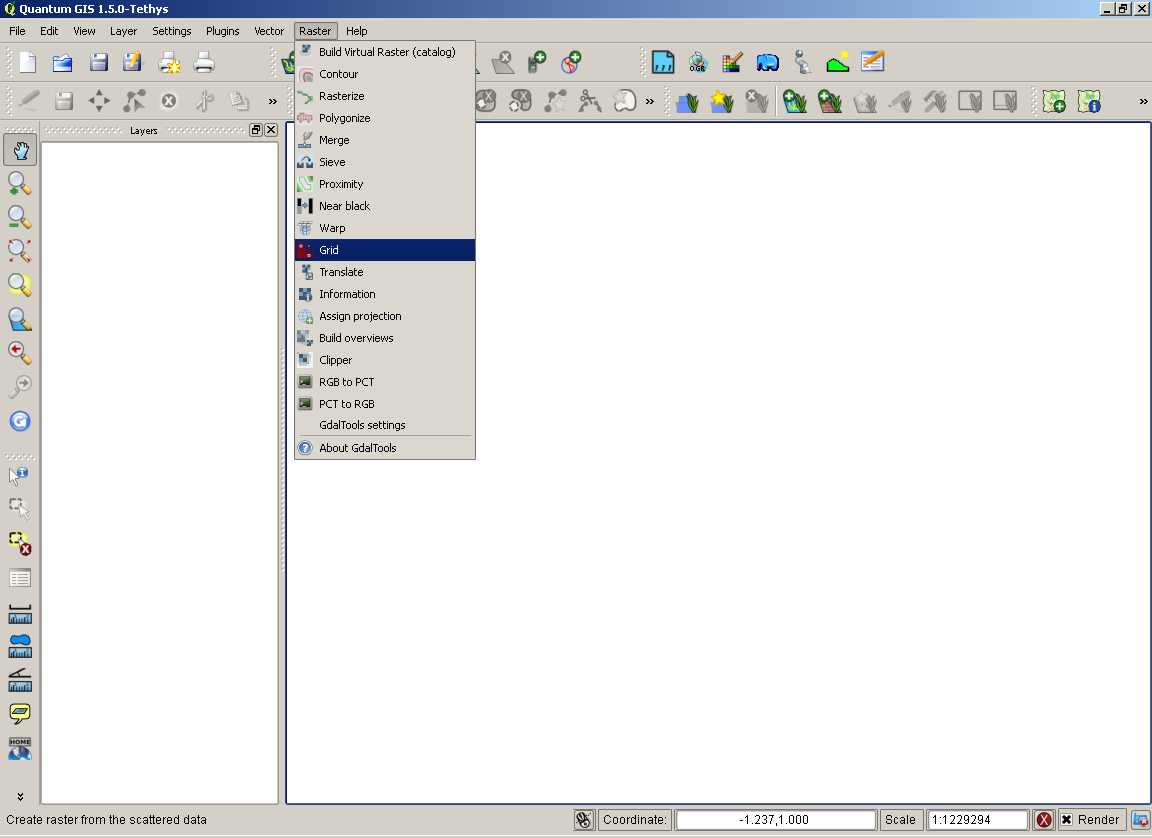
\includegraphics[clip=true, width=12cm]{plugins_gdaltools_images/raster_menu}
   \caption{\label{gdaltools_menu}Меню \emph{Растр} \wincaption}
\end{figure}

\subsection{Примеры}\label{gdal_examples}
Ниже приведены несколько примеров использования инструментов из состава модуля.
\subsubsection{Получение информации о растре}
\begin{figure}[ht]
   \centering
   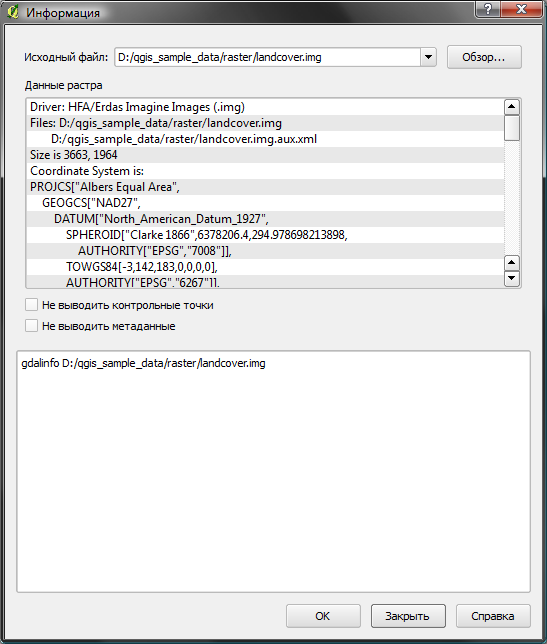
\includegraphics[clip=true, width=12cm]{plugins_gdaltools_images/gdalinfo}
   \caption{\label{gdalinfo}Диалог \emph{Информация} \wincaption}
\end{figure}

\subsubsection{Создание изолиний}
В данном примере будут построены изолинии на основе фрагмента данных SRTM.
\begin{figure}[ht]
   \centering
   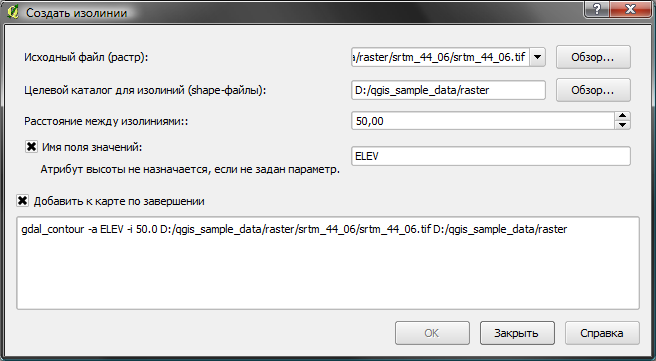
\includegraphics[clip=true, width=12cm]{plugins_gdaltools_images/gdal_contour}
   \caption{\label{gdal_contour} Диалог \emph{Создать изолинии} \wincaption}
\end{figure}
в результате получаем:
\begin{figure}[ht]
   \centering
   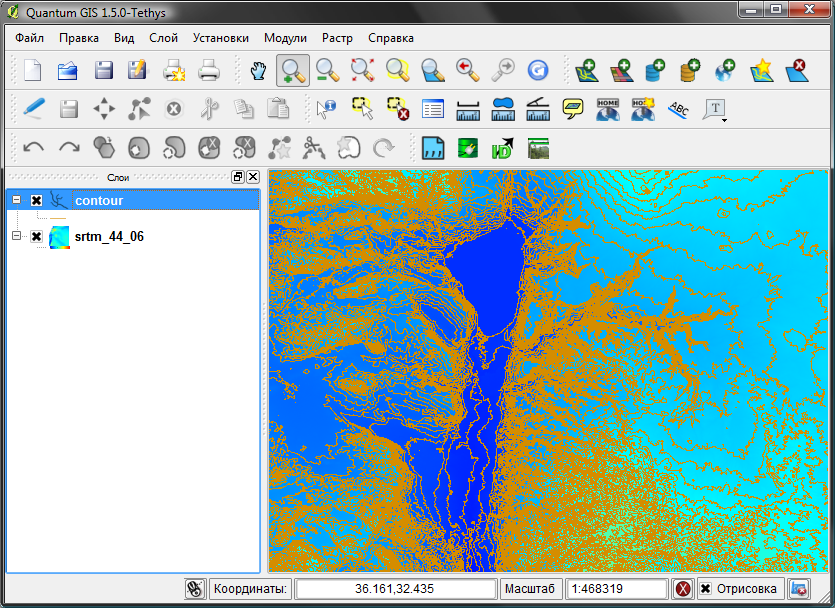
\includegraphics[clip=true, width=12cm]{plugins_gdaltools_images/qgis_contours}
   \caption{\label{gdal_contour} Итоговый слой изолиний \wincaption}
\end{figure}

\subsubsection{Использование инструмента <<Трансформировать проекцию>> для перепроецирования растра}
На скриншоте представлено диалоговое окно перепроецирования растра
растительного покрова из исходной равноплощадной проекции Альберса для Аляски (из набора данных QGIS
sample dataset) в географическую проекцию на эллипсоиде WGS-84 (Lon/Lat WGS-84) (EPSG:4326).
\begin{figure}[ht]
   \centering
   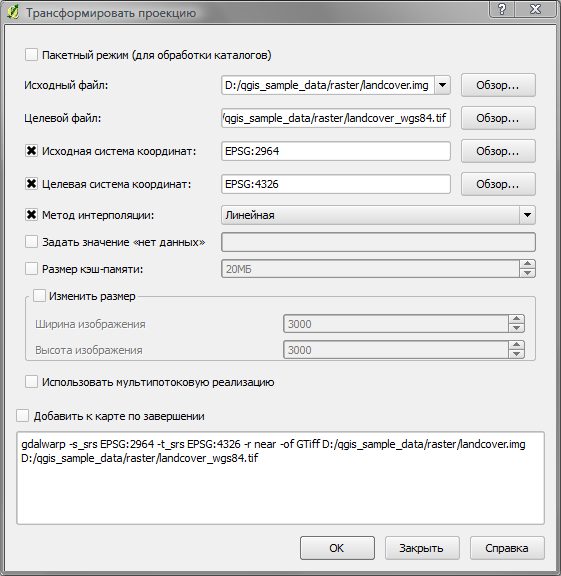
\includegraphics[clip=true, width=12cm]{plugins_gdaltools_images/gdalwarp}
   \caption{\label{gdalwarp} Диалог \emph{Трансформировать проекцию} \wincaption}
\end{figure}

\FloatBarrier
